\subsection{\color{ForestGreen}Parse Trees, Ambiguity}
\subsubsection{Definitions}
\begin{itemize}
    \item Parse tree: Leaves are terminals, Interior nodes are variables, root is start symbol, children are labeled by the right side of a production for the parent.
    \begin{Figure}
        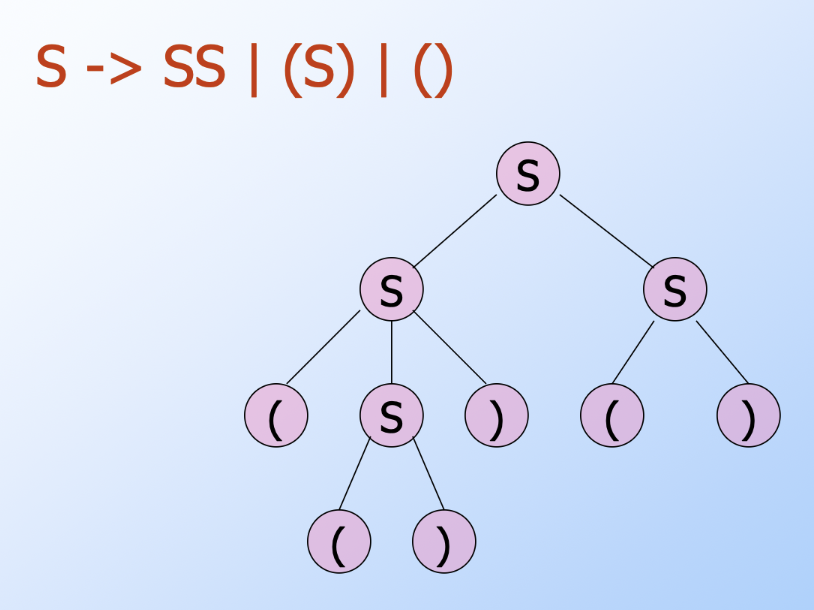
\includegraphics[width=0.5\textwidth]{figures/parsetree.png}
    \end{Figure}
    \item Yield: concatenation of the labels of the leaves in left-to-right order.
    \item A CFG is said to be \textit{right-linear} if each production body has at most one variable and that variable is at the right end, i.e. all productions of a {right-linear} grammar are of the form $A \rightarrow{}wB$ or $A\rightarrow{}w.$
    \item A CFG is \textbf{ambiguous} if there is a string in the language that is the yield of two or more parse trees. Equivalently, if there are two or more leftmost derivations for a string.  
    \item \textbf{Inherent Ambiguity}: every grammar for the language is ambiguous. 
\end{itemize}
\subsubsection{Results}
\begin{itemize}
    \item \textit{Right-linear} $\iff $ \textit{regular language}. Proof: $(\implies)$ Construct an $\epsilon$-NFA that simulates leftmost derivations using its state to represent the lone variable in the current left-sentential form. $(\impliedby)$ Start with a DFA and let the variables of the grammar represent states.
    \item The recursive inference procedure determines that terminal string $w$ is in the language of variable $A$ $\iff A \overset{*}{\implies} w \iff A \overset{*}{\implies}_{lm} w$ $\iff A \overset{*}{\implies}_{rm}w \iff $ there is a parse tree with root $A$ and yield $w.$
    \item CFG $G$ is ambiguous $\iff$ There is a string in the language that has two different left/rightmost derivations.
    \item There is no algorithm that can tell whether a CFG is ambiguous (\textit{undecidable}).
\end{itemize}